% For LaTeX-Box: root = stat105_F15_exam1B.tex 
%%%%%%%%%%%%%%%%%%%%%%%%%%%%%%%%%%%%%%%%%%%%%%%%%%%%%%%%%%%%%%%%%%%%%%%%%%%%%%%%
%  File Name: stat105_F15_exam1B.tex
%  Purpose:
%
%  Creation Date: 24-09-2015
%  Last Modified: Thu Oct  1 00:18:14 2015
%  Created By:
%%%%%%%%%%%%%%%%%%%%%%%%%%%%%%%%%%%%%%%%%%%%%%%%%%%%%%%%%%%%%%%%%%%%%%%%%%%%%%%%
\documentclass[addpoints]{examsetup}

\usepackage{etoolbox}
\usepackage{tikz,pgfplots}

%% For LaTeX-Box: root = stat105_exam1_info.tex 
%%%%%%%%%%%%%%%%%%%%%%%%%%%%%%%%%%%%%%%%%%%%%%%%%%%%%%%%%%%%%%%%%%%%%%%%%%%%%%%%
%  File Name: stat105_exam1_info.tex
%  Purpose:
%
%  Creation Date: 24-09-2015
%  Last Modified: Thu Sep 24 13:51:36 2015
%  Created By:
%%%%%%%%%%%%%%%%%%%%%%%%%%%%%%%%%%%%%%%%%%%%%%%%%%%%%%%%%%%%%%%%%%%%%%%%%%%%%%%%
\newcommand{\course}[1]{\ifstrempty{#1}{STAT 105}{STAT 105, Section #1}}
\newcommand{\sectionNumber}{B}
\newcommand{\examDate}{October 1, 2015}
\newcommand{\semester}{FALL 2015}
\newcommand{\examNumber}{II}

\newcommand{\examTitle}{Exam \examNumber}

\runningheader{\course{\sectionNumber}}{Exam \examNumber}{\examDate}
\runningfooter{}{}{Page \thepage of \numpages}

\newcommand{\examCoverPage}{
   \begin{coverpages}
   \centering
   {\bfseries\scshape\Huge Exam I \par}
   \vspace{1cm}
   {\bfseries\scshape\LARGE \course{\sectionNumber} \par}
   {\bfseries\scshape\LARGE \semester \par}

   \vspace{2cm}

   \fbox{\fbox{\parbox{5.5in}{\centering 

      \vspace{.25cm} 
      
      {\bfseries\Large Instructions} \\

      \vspace{.5cm} 

      \begin{itemize}
         \item  The exam is scheduled for 80 minutes, from 8:00 to 9:20 AM. At 9:20 AM the exam will end.\\
         \item  A forumula sheet is attached to the end of the exam. Feel free to tear it off.\\
         \item  You may use a calculator during this exam.\\
         \item  Answer the questions in the space provided. If you run out of room, continue on the back of the page. \\
         \item  If you have any questions about, or need clarification on the meaning of an item on this exam, please ask your instructor. No other form of external help is permitted attempting to receive help or provide help to others will be considered cheating.\\
         \item  {\bfseries Do not cheat on this exam.} Academic integrity demands an honest and fair testing environment. Cheating will not be tolerated and will result in an immediate score of 0 on the exam and an incident report will be submitted to the dean's office.\\
      \end{itemize}

   }}}

   \vspace{2cm}

   \makebox[0.6\textwidth]{Name:\enspace\hrulefill}

   \vspace{1cm}

   \makebox[0.6\textwidth]{Student ID:\enspace\hrulefill}
   \end{coverpages}

}


\newcommand{\course}[1]{\ifstrempty{#1}{STAT 305}{STAT 305, Section #1}}
\newcommand{\sectionNumber}{3}
\newcommand{\examDate}{October 17, 2019}
\newcommand{\semester}{FALL 2019}
\newcommand{\examNumber}{II}

%%%%%%%%%%%%%%%%%%%%%%%%%%%%%%%%%%%%%%%%%%%%%%%%%%%%%%%%%%%%%%%%%%%%%%%%%%%%%%%%

\usepackage{Sweave}
\begin{document}
\Sconcordance{concordance:stat305_q2.tex:stat305_q2.Rnw:%
1 23 1 1 0 3 1 1 6 25 1 1 17 2 1 1 7 1 2 165 1}


%-- : R code (Code in Document)


\examCoverPage

\begin{questions}



\question

Professional engineers often encounter issues relating to \textit{human resources} as they advance in their careers
(building a better team of employees is after all not too different than improving any other system, at least on paper).
However, many of the "laws" governing human behavior are very different than the strict laws of physics.
For instance, a phenomenon known as the Dunning-Kruger effect states that for a given skill incompetent people will
\begin{itemize}
   \item fail to recognize their own lack of skill
   \item fail to recognize genuine skill in others
   \item fail to recognize the extremity of their inadequacy
   \item recognize and acknowledge their own lack of skill, after they are exposed to training for that skill
\end{itemize}

A group of 50 job applicants are asked to estimate their skill in technical writing. 
They are told they will be taking a test with a mean score of 50 and asked to guess what their score will be.
Then they are given the test and get an actual score. 

%-- : R code (Code in Document)

The results are depicted below (using the actual score on the x-axis):
\begin{center}
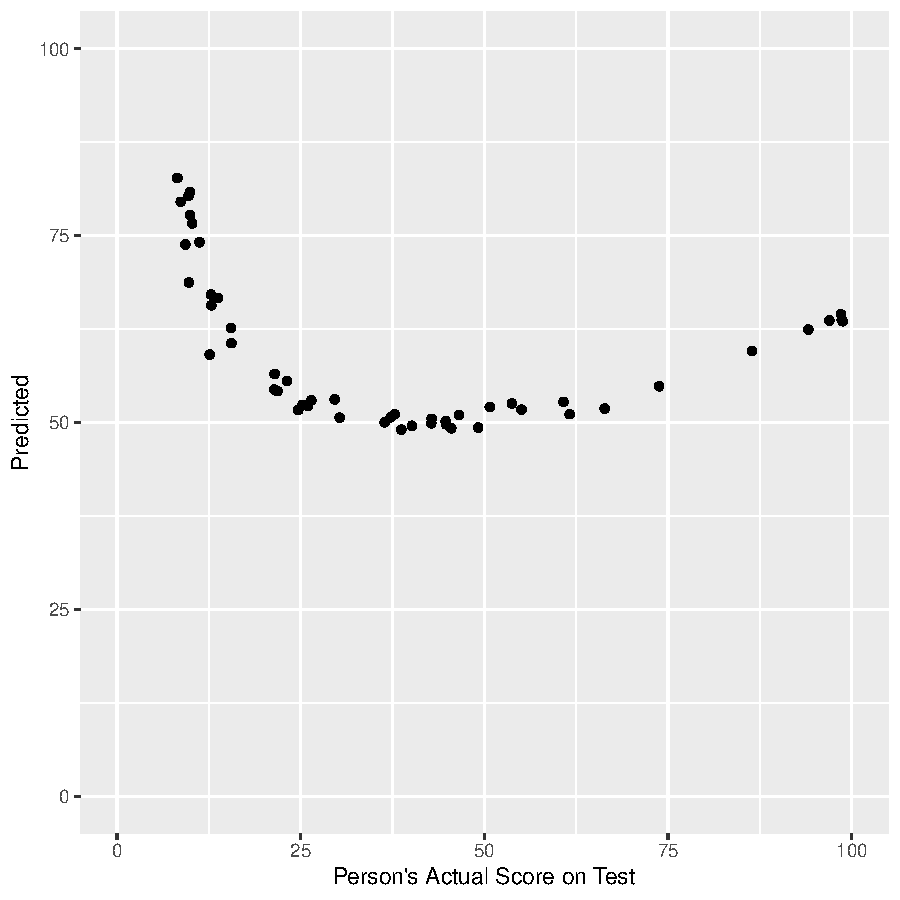
\includegraphics{stat305_q2-003}
\end{center}
\pagebreak
Here are some summaries of the data (again using the actual score as the x-value and the person's evaluation of their score as the y-value):

$$
   \sum_{i=1}^{50} x_i = 1922 \hspace{3cm} \sum_{i=1}^{50} x_i^2 = 110659 \\
$$

$$
   \sum_{i=1}^{50} y_i = 2954 \hspace{3cm} \sum_{i=1}^{50} y_i^2 = 179606 \\
$$

$$
   \sum_{i=1}^{50} x_i y_i = 108893
$$

\begin{parts}
   \part Using the summaries above, fit a linear relationship between \textbf{the actual score} (x) and \textbf{the guessed score} (y). 
   \begin{subparts}
      \subpart[5] Write the equation of the fitted linear relationship. 
      
      \hfill \fbox{ \textcolor[rgb]{1.00,1.00,1.00}{$\bigcap$} \hskip -0.4cm $\hat y =$ \hspace{10cm}}
      \vspace{7cm}
      \subpart[5] Find and interpret the value of $R^2$ for the fitted linear relationship.
                  \hfill \fbox{ \textcolor[rgb]{1.00,1.00,1.00}{$\bigcap$} \hskip-0.4cm $R^2=$ \hspace{2cm}}

      \vspace{7cm}
      \subpart[5] Using the fitted line, what do we suppose a person will guess their score will be if they actually scored a 40.14.
      
      
            \hfill \fbox{ \textcolor[rgb]{1.00,1.00,1.00}{$\bigcap$} \hskip -0.4cm $\hat y =$ \hspace{10cm}}

      \vspace{3cm}
      \subpart[2] A person who scored a 40.14 on the test predicted that they would score 49.56. What is the residual for this person using the linear relationship?
      
      
                  \hfill \fbox{ \textcolor[rgb]{1.00,1.00,1.00}{$\bigcap$} \hskip -0.4cm $e =$ \hspace{5cm}}

      \vspace{2cm}
      
      
   \end{subparts}

 

   \part The JMP output below comes from fitting a quadratic model using the actual score ("\verb!actual_score!") and the square of the actual score (\verb!actual_score^2!).

   \centerline{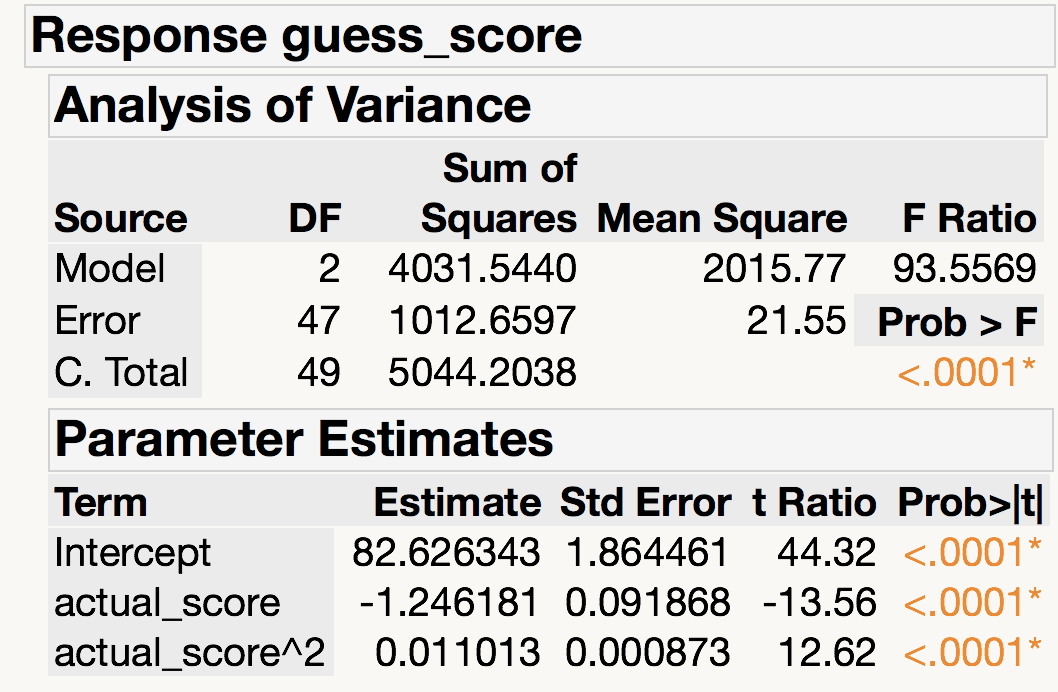
\includegraphics[scale=.2]{FitDK}}

   \begin{subparts}
      \subpart[5] Write the equation of the fitted quadratic relationship.
      
\hfill \fbox{ \textcolor[rgb]{1.00,1.00,1.00}{$\bigcap$} \hskip -0.4cm $\hat y =$ \hspace{10cm}}

      \vspace{1cm}
      \subpart[5] Find and interpret the value of $R^2$ for the fitted quadratic relationship.
                        \hfill \fbox{ \textcolor[rgb]{1.00,1.00,1.00}{$\bigcap$} \hskip-0.4cm $R^2=$ \hspace{3cm}}

      \vspace{5cm}
\pagebreak      
      \subpart[5] Using the fitted quadratic relationship, what do we suppose a person will guess their score will be if they actually scored a 98.74.
      
                  \hfill \fbox{ \textcolor[rgb]{1.00,1.00,1.00}{$\bigcap$} \hskip -0.4cm $\hat y =$ \hspace{10cm}}

      \vspace{2cm}
     
      \subpart[2] A person who scored a 98.74 on the test predicted that they would score 63.55. What is the residual for this person using the quadratic relationship?
      
\hfill \fbox{ \textcolor[rgb]{1.00,1.00,1.00}{$\bigcap$} \hskip -0.4cm $e =$ \hspace{5cm}}

      \vspace{2cm}
   \end{subparts}
\end{parts}

\question
Suppose the following is the probability distribution for $X$. 
 \begin{table}[h!]
     \centering
     \begin{tabular}{llllll}
        \hline
         x  & -2  & 0 &  1  & 2 & 3     \\\hline \hline
         f(x) & 0.1 &  a & 0.2  & 0.2 &  0.3  \\\hline \hline

     \end{tabular}
  \end{table}
         \begin{subparts}
               \subpart[3] Find the value of $a$ that makes this a valid probability distribution.
                                       \hfill \fbox{ \textcolor[rgb]{1.00,1.00,1.00}{$\bigcap$} \hskip-0.4cm $a=$ \hspace{2cm}}
         
               \vspace{4cm}
               
               \subpart[6] Calculate the expected value and the standard deviation of $X$.
                     \vskip
                     \hfill \fbox{ \textcolor[rgb]{1.00,1.00,1.00}{$\bigcap$} \hskip
                     -0.4cm E(X)= \hspace{3cm}}
                     \vskip
                     \hfill \fbox{ \textcolor[rgb]{1.00,1.00,1.00}{$\bigcap$} \hskip
                     -0.4cm SD(X)=\hspace{2.9cm}}
                     \vskip
                     
               \vspace{5cm}   
               
               \subpart[2] Find the probability that $P(\vert{X}\vert =2)$
               \hfill \fbox{$P(\vert{X}\vert =2)=$\hspace{3cm}} 
               \vspace
               
               
         \end{subparts}
         
\pagebreak

\question
As the discussion in the class, King Joffrey was poisoned and Tyrion was found guilty  for his death. Tyrion then decided to let the gods decide his fate and demanded a trial by combats. Then it was supposed to have five completely independent combats to decide on his guilt or innnocence. The one who fought for him (his combatant) had $p= 0.7$ probability of success in each combat.  Let $X$ be the random variable associated with the number of combats his combatant wins out of the five combats.

         \begin{subparts}
               \subpart[2] Precisely specify the probability distribution associated with this trial.
               \vspace{2cm}
               
               \subpart[3] What is the probability that his combatant wins all combats?
               \hfill \fbox{$p=$ \hspace{3cm}}
               \vspace{4cm}
               
               \subpart[3] What is the probability that his combatant wins at least two combats?
               \hfill \fbox{$p=$ \hspace{3cm}}
               \vspace{6cm}       
               
               \subpart[2] What is the expected value of this random variable $X$?
               \hfill \fbox{$E(X)=$ \hspace{3cm}}
               \vspace{2cm}       
                              
               \subpart[2] What is the variance  of this random variable $X$?
               \hfill \fbox{$Var(X)=$ \hspace{3cm}}
               \vspace{2cm}          
         
         \end{subparts}

\pagebreak
\question
Suppose that an eddy current nondestructive evaluation technique for identifying cracks in critical metal parts has a probability of about $.20$ of detecting a single crack of length $.003$in. in a certain material. Let $Y$ be the number of specimens inspected in order to obtain the first crack detection.
\vspace{1cm}
         \begin{subparts}
                  \subpart[2] Precisely state the distribution of $Y$, giving the values of any parameters necessary.
                  \vspace{2cm}
                  
                  \subpart[3] Find the probability that $P(Y = 5)$
                  \hfill \fbox{$P(Y = 5)=$ \hspace{3cm}}
                  \vspace{5cm}
                  
                  \subpart[3] Find the probability that $P(Y \le 4)$
                  \hfill \fbox{$P(Y \le 4)=$ \hspace{3cm}}
                  \vspace{5cm}
                  
                  \subpart[2] What is $\text{E}Y$?
                  \hfill \fbox{$\text{E}(Y)= $ \hspace{3cm}}
                  \vspace{2cm}
                  
                  
                  \subpart[2] What is $SD{(Y)}$ (the standard deviation of $Y$)?
                  \hfill \fbox{$\text{SD(Y)}= $ \hspace{3cm}}
                  \vspace{2cm}                                    
                           
         \end{subparts}

\end{questions}

\end{document}
